\chapter{$\PT$-Symmetric Optics}
\label{ch:pt-symmetric}

\begin{chapterlead}
Among all non-Hermitian photonic systems, those with parity--time ($\PT$)
symmetry occupy a special place. A $\PT$-symmetric structure has a
refractive-index profile that satisfies $n(\rr) = n^*(-\rr)$: the real
part is symmetric and the imaginary part is antisymmetric under spatial
inversion. Gain and loss are balanced, and the system can exhibit a
$\PT$ phase transition~\cite{elganainy2007theory}---from a regime with entirely real
eigenfrequencies to one with complex conjugate pairs---controlled by a
single parameter. The $\PT$-symmetry condition is derived from the
Helmholtz equation, followed by the transfer-matrix theory for $\PT$
Bragg gratings and the associated phenomena: spontaneous
$\PT$-symmetry breaking, unidirectional invisibility, and the connection
to exceptional points.
\end{chapterlead}


%% ================================================================
\section{The $\PT$-symmetry condition}
\label{sec:pt-condition}

\subsection{Parity and time reversal in Maxwell's equations}
\label{ssec:pt-maxwell}

The parity operator $\mathcal{P}$ acts by spatial inversion:
$\mathcal{P}\EE(\rr) = -\EE(-\rr)$, $\mathcal{P}\HH(\rr) = \HH(-\rr)$
(the signs follow from the vector and pseudovector character of $\EE$ and
$\HH$). The time-reversal operator $\mathcal{T}$ acts by complex
conjugation on the frequency-domain fields: $\mathcal{T}\EE(\rr) =
\EE^*(\rr)$, which reverses the sign of $\omega$ and exchanges incoming
and outgoing waves.

A system described by a spatially varying permittivity $\epsr(\rr)$ is
$\PT$-symmetric if the combined operation $\PT$ leaves the Helmholtz
equation invariant. For the scalar Helmholtz equation
\begin{equation}
 -\nabla^2\psi(\rr) = \frac{\omega^2}{c^2}\,n^2(\rr)\,\psi(\rr),
 \label{eq:helmholtz-scalar}
\end{equation}
the $\PT$ transformation maps $\psi(\rr) \to \psi^*(-\rr)$ and requires
\begin{equation}
 \boxed{n^2(\rr) = [n^2(-\rr)]^*,}
 \label{eq:pt-n-condition}
\end{equation}
or equivalently for the permittivity:
$\epsr(\rr) = \epsr^*(-\rr)$. This means
\begin{equation}
 \epsr'(\rr) = \epsr'(-\rr), \qquad
 \epsr''(\rr) = -\epsr''(-\rr):
 \label{eq:pt-eps-parts}
\end{equation}
the real part of the permittivity is spatially even and the imaginary part
is spatially odd. Regions of gain and loss are arranged as mirror images.

\subsection{$\PT$ symmetry does not mean Hermiticity}
\label{ssec:pt-not-hermitian}

A $\PT$-symmetric system has complex $\epsr(\rr)$; it is not Hermitian.
However, the balance of gain and loss allows the eigenfrequencies to be
real over a range of parameters---the \emph{$\PT$-symmetric phase}. The
eigenfrequencies become complex only when the gain--loss contrast exceeds
a critical threshold: the $\PT$-breaking transition, which occurs at an
exceptional point (Chapter~\ref{ch:exceptional-points}).

It is worth stating exactly what $\PT$ symmetry does and does not
guarantee:
\begin{itemize}
 \item It \emph{does} guarantee that eigenvalues come in conjugate
 pairs or are real: if $\omtil$ is an eigenvalue, so is $\omtil^*$.
 \item It \emph{does not} guarantee that all eigenvalues are real.
 The transition from real to complex eigenvalues is spontaneous
 symmetry breaking: the eigenstates cease to be simultaneous
 eigenstates of $\PT$.
 \item It \emph{does not} guarantee stability. Even in the
 $\PT$-symmetric phase, the non-normality of the Hamiltonian can
 produce large transient growth
 (Section~\ref{sec:matrix-exp}).
\end{itemize}

\subsection{$\PT$ symmetry from the energy inner product}
\label{ssec:pt-energy}

The relation between $\PT$ symmetry and the energy inner product of
Chapter~\ref{ch:energy-inner} can be made precise. The Maxwell
curl--curl operator $\hat{\Theta}$ is self-adjoint with respect to
the $\epsr$-weighted inner product when $\epsr$ is real. When
$\epsr$ is complex but satisfies $\epsr(\rr) = \epsr^*(-\rr)$, the
operator is no longer self-adjoint in the standard inner product, but
it commutes with the antilinear operator $\PT$:
\begin{equation}
 [\hat{\Theta},\,\PT] = 0
 \qquad\text{when}\qquad
 \epsr(\rr) = \epsr^*(-\rr).
 \label{eq:theta-pt-commute}
\end{equation}
This commutation replaces self-adjointness as the organizing symmetry
of the spectrum. Bender and Boettcher first recognized this structure
in quantum mechanics; in photonics, it descends directly from the
Maxwell equations.


%% ================================================================
\section{$\PT$ phase transition in the two-mode model}
\label{sec:pt-two-mode}

The simplest $\PT$-symmetric system is a pair of coupled resonances with
equal and opposite gain/loss rates, described by the effective Hamiltonian
\begin{equation}
 H_{\PT} =
 \begin{pmatrix}
 \omega_0 + i\gamma & \kappa \\
 \kappa & \omega_0 - i\gamma
 \end{pmatrix},
 \label{eq:pt-hamiltonian}
\end{equation}
where $\gamma > 0$ is the gain/loss rate and $\kappa > 0$ is the real
coupling. The eigenvalues are
\begin{equation}
 \omtil_\pm = \omega_0 \pm \sqrt{\kappa^2 - \gamma^2}.
 \label{eq:pt-eigenvalues}
\end{equation}

\begin{figure}[t]
 \centering
 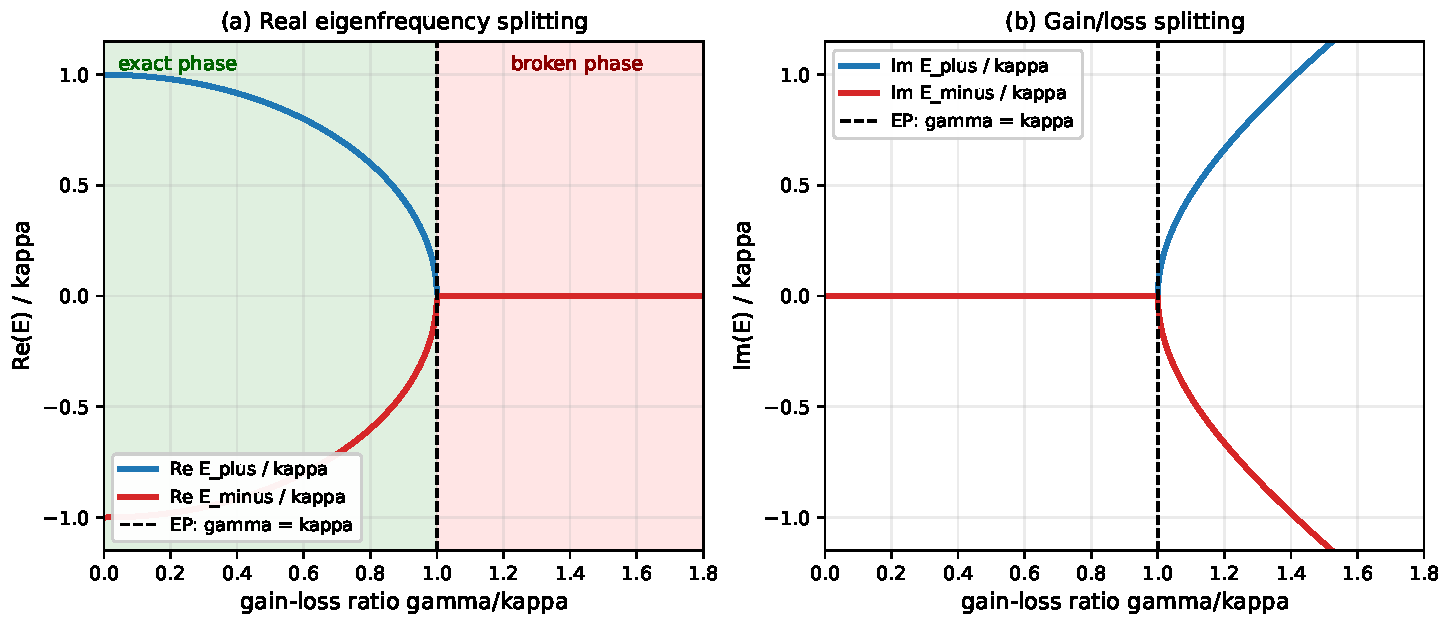
\includegraphics[width=0.85\linewidth]{figures/fig_f09_pt_phase_diagram.pdf}
 \caption{$\PT$ phase transition in the two-mode model.
 (a)~Real parts of the eigenvalues: in the exact $\PT$-symmetric
 phase ($\gamma < \kappa$, green shading) both eigenfrequencies are
 real and split; in the broken phase ($\gamma > \kappa$, red shading)
 they coalesce.
 (b)~Imaginary parts: zero throughout the exact phase, then
 bifurcating symmetrically in the broken phase. The exceptional point
 at $\gamma = \kappa$ (dashed line) marks the phase boundary where
 eigenvalues and eigenvectors simultaneously coalesce.}
 \label{fig:pt-phase-diagram}
\end{figure}

\paragraph{$\PT$-symmetric phase ($\gamma < \kappa$).}
The square root is real, and the eigenfrequencies $\omtil_\pm$ are both
real despite the non-Hermiticity of $H_{\PT}$. The modes are extended
over both resonators with equal gain and loss, so each mode experiences
zero net amplification.

\paragraph{$\PT$-broken phase ($\gamma > \kappa$).}
The square root becomes imaginary, and the eigenfrequencies form a complex
conjugate pair:
$\omtil_\pm = \omega_0 \pm i\sqrt{\gamma^2 - \kappa^2}$. One mode is
amplified, the other is attenuated. The gain--loss contrast has overcome
the coupling.

\paragraph{The exceptional point ($\gamma = \kappa$).}
At the transition, the eigenvalues coalesce at $\omega_0$ and the
eigenvectors merge. This is an EP$_2$ of exactly the type analyzed in
Section~\ref{sec:ep2}.

\subsection{Coupled-mode derivation from Maxwell fields}
\label{ssec:pt-cmt-maxwell}

The two-mode Hamiltonian~\eqref{eq:pt-hamiltonian} is not postulated
but derived from the Maxwell equations via the coupled-mode formalism of
Chapter~\ref{ch:maxwell-coupled-modes}. Consider two weakly coupled
cavities with identical real permittivity profiles but opposite imaginary
parts: cavity~A has $\varepsilon_A = \varepsilon_0 + i\kappa_I$ and cavity~B
has $\varepsilon_B = \varepsilon_0 - i\kappa_I$. The QNM framework of
Chapter~\ref{ch:qnm} gives each isolated cavity the same resonance
frequency $\omega_0$ but opposite imaginary corrections:
\begin{equation}
 \omtil_A = \omega_0 - i\gamma_{\mathrm{rad}} - i\gamma_{\mathrm{mat}},
 \qquad
 \omtil_B = \omega_0 - i\gamma_{\mathrm{rad}} + i\gamma_{\mathrm{mat}},
 \label{eq:pt-isolated-modes}
\end{equation}
where $\gamma_{\mathrm{rad}}$ is the (common) radiative decay rate and
$\gamma_{\mathrm{mat}} \propto \kappa_I$ is the material loss/gain rate
for the sign convention used here. Thus cavity~A is the lossy partner
and cavity~B is the gain partner for $\kappa_I>0$.
When the two cavities are brought into evanescent proximity, the overlap
integral of the reaction inner product
(Section~\ref{sec:reaction}) gives a coupling matrix element
$\kappa$ that is real and symmetric for reciprocal media. The
resulting $2\times 2$ effective Hamiltonian is exactly of the
form~\eqref{eq:pt-hamiltonian}, after subtracting the common offset
$\omega_0-i\gamma_{\mathrm{rad}}$ and identifying
$\gamma = \gamma_{\mathrm{mat}}$ up to the ordering of the two basis
states.

The Maxwell derivation shows explicitly that the $\PT$ condition for the
two-mode model---equal and opposite imaginary diagonal entries---is a
consequence of the $\PT$ condition for the permittivity, not an
independent postulate. It also reveals when the two-mode description
breaks down: when the coupling $\kappa$ is comparable to the mode
spacing, or when higher-order modes contribute significantly.


%% ================================================================
\section{Transfer-matrix theory for $\PT$ gratings}
\label{sec:pt-transfer}

\subsection{The 1D $\PT$-symmetric Bragg grating}
\label{ssec:pt-bragg}

Consider a one-dimensional periodic structure with refractive index
\begin{equation}
 n(x) = n_0 + \Delta n\cos(2\pi x/\Lambda)
 + i\Delta n_I\sin(2\pi x/\Lambda),
 \label{eq:pt-grating-n}
\end{equation}
where $n_0$ is the background index, $\Delta n$ is the real modulation
depth, $\Delta n_I$ is the imaginary modulation depth, and $\Lambda$ is
the period. This profile satisfies $n(x) = n^*(-x)$: it is
$\PT$-symmetric. When $\Delta n = 0$ and only the imaginary modulation
remains, the grating is purely gain--loss modulated.

\subsection{Transfer matrix for one period}
\label{ssec:pt-transfer-matrix}

Each period of the grating is a layered structure that can be described
by a $2\times 2$ transfer matrix $\Tmat$ relating the forward- and
backward-propagating wave amplitudes on the left to those on the right
(Appendix~\ref{app:transfer}). For a grating of $N$ periods, the total
transfer matrix is $\Tmat^N$.

The scattering matrix is obtained from $\Tmat$ by the standard conversion.
The reflection and transmission coefficients are~\cite{lin2011unidirectional}
\begin{equation}
 r_L = -\frac{T_{21}}{T_{22}}, \quad
 r_R = \frac{T_{12}}{T_{22}}, \quad
 t = \frac{1}{T_{22}},
 \label{eq:pt-transfer-to-scatter}
\end{equation}
where $T_{ij}$ are the elements of $\Tmat^N$.

\subsection{Example: a $\PT$ bilayer}
\label{ssec:pt-bilayer-example}

To make the transfer-matrix formalism concrete, consider the simplest
$\PT$ structure: a single unit cell with a loss slab
($n_1 = 3.0 + 0.05\,i$, thickness $d = 200\;\mathrm{nm}$) and a gain
slab ($n_2 = 3.0 - 0.05\,i$, same thickness). At wavelength
$\lambda = 1550\;\mathrm{nm}$, the propagation phase per slab is
$\phi = n k_0 d \approx 2.43 + 0.041\,i$ rad.

The single-slab propagation matrix is (Appendix~\ref{app:transfer})
\begin{equation}
 M_j = \begin{pmatrix} e^{in_j k_0 d} & 0 \\ 0 & e^{-in_j k_0 d} \end{pmatrix},
 \label{eq:pt-slab-matrix}
\end{equation}
and the interface matrix between slabs with indices $n_a$ and $n_b$ is
$I_{ab} = \tfrac{1}{2n_b}\bigl(\begin{smallmatrix} n_b+n_a & n_b-n_a
\\ n_b-n_a & n_b+n_a \end{smallmatrix}\bigr)$.
The unit-cell transfer matrix is
$\Tmat_{\mathrm{cell}} = I_{2,\mathrm{out}} \cdot M_2 \cdot I_{12}
\cdot M_1 \cdot I_{\mathrm{in},1}$.

For this example, the trace of $\Tmat_{\mathrm{cell}}$ is nearly real
and satisfies $|\tfrac{1}{2}\tr\Tmat_{\mathrm{cell}}| < 1$: the system is
in the $\PT$-symmetric phase. The left and right reflection
coefficients are
\begin{equation}
 |r_L| \approx 0.033, \qquad |r_R| \approx 0.034, \qquad
 |t| \approx 1.002,
 \label{eq:pt-bilayer-numbers}
\end{equation}
showing near-unit transmission with slightly asymmetric reflection.
The asymmetry grows with the number of unit cells $N$.

\begin{figure}[t]
 \centering
 
\includegraphics[width=0.98\textwidth]{fig_f9_pt_bilayer_spectra.pdf}
 \caption{Transfer-matrix spectra of a finite stack built from $\PT$-symmetric bilayer unit cells. The unit cell is the loss--gain pair used in this example, repeated $N=6$ times and embedded in air. Panel (a) shows the wavelength dependence of transmission $T=|t|^2$ and the mean reflectance $\bar R=(R_L+R_R)/2$; because the stack contains gain and loss, these are scattering intensities rather than a unitary energy partition. The small left--right difference is not visually useful on the logarithmic spectrum, so panel (b) plots the directional reflection asymmetry $A_R(\lambda)=(R_R-R_L)/(R_R+R_L)$ directly; negative $A_R$ means stronger reflection for left incidence. Panel (c) fixes $\lambda=1550\,\mathrm{nm}$ and varies the gain--loss index contrast $\kappa_I$, showing $A_R(1550\,\mathrm{nm})$ and the transmission $T$ as functions of gain/loss strength.}
 \label{fig:pt-bilayer-spectra}
\end{figure}

\subsection{Unidirectional invisibility}
\label{ssec:unidirectional}

Suitably designed $\PT$ Bragg gratings can exhibit
\emph{unidirectional invisibility}: at a scattering exceptional point or
anisotropic transmission resonance, the grating can be transparent from
one side ($r_L = 0$, $|t| = 1$) while remaining reflective from the other
side ($r_R \neq 0$)~\cite{lin2011unidirectional}. This is not a generic
consequence of every $\PT$-breaking point; it requires the grating
parameters and operating frequency to satisfy the corresponding
scattering condition.

The physical mechanism can be understood from the transfer-matrix
eigenvalue structure. At the EP, one eigenvalue has unit modulus
while the other is its inverse: $\lambda_+ = 1/\lambda_-^*$. The
corresponding eigenvectors correspond to forward- and backward-traveling
Bloch waves. For incidence from one side, the field couples
predominantly to the non-growing eigenstate and passes through with
unit transmission and zero reflection; for incidence from the other
side, the field excites the growing eigenstate, producing finite
reflection.

This asymmetry is not a violation of reciprocity---the transmission
coefficient is the same from both sides ($t_L = t_R$ for a reciprocal
medium)---but the reflection coefficients differ:
$|r_L| \neq |r_R|$. In a lossless reciprocal one-dimensional grating,
$|r_L| = |r_R|$ follows from the combination of reciprocity and flux
conservation. In the $\PT$-symmetric case, flux conservation is broken
and the two reflection magnitudes can differ even though the
transmission amplitude remains reciprocal.

\subsection{Spectral features near the Bragg condition}
\label{ssec:pt-bragg-spectrum}

The most dramatic $\PT$ effects occur near the Bragg condition
$\lambda = 2 n_0 \Lambda$, where the stop band of a conventional
(Hermitian) grating is located. In the $\PT$-symmetric grating:
\begin{itemize}
 \item Below the EP: the stop band splits into two narrower bands
 separated by a transmission peak at the Bragg wavelength.
 \item At the EP: the two bands merge, and the central peak becomes
 a unity-transmission point with divergent group delay---a critical
 slowing of light.
 \item Above the EP: the merged band becomes an amplification window
 for one scattering channel and an absorption window for the other.
\end{itemize}

These features have been observed experimentally in coupled-fiber
systems and semiconductor gratings, confirming the transfer-matrix
predictions quantitatively.

\begin{takeaway}[$\PT$ gratings break reflection symmetry, not reciprocity]
A $\PT$-symmetric Bragg grating is reciprocal ($t_L = t_R$) but not
unitary ($|r_L| \neq |r_R|$). The asymmetric reflection is a direct
consequence of balanced gain and loss, and it vanishes in the Hermitian
limit ($\Delta n_I \to 0$). This distinction between reciprocity and
unitarity echoes the general principle established in
Section~\ref{sec:reciprocity}.
\end{takeaway}


%% ================================================================
\section{$\PT$ symmetry of the scattering matrix}
\label{sec:pt-smatrix}

For a one-dimensional two-port $\PT$-symmetric structure with the port
basis ordered by left and right incidence, the scattering matrix satisfies
a
fundamental relation derived by Chong, Ge, and
Stone~\cite{chong2010symmetry}:
\begin{equation}
 (\PT)\,\Smat(\omega^*)\,(\PT) = \Smat^{-1}(\omega).
 \label{eq:pt-s-relation}
\end{equation}
For real frequencies, this implies
\begin{equation}
 |\det\Smat(\omega)| = 1:
 \label{eq:det-s-unit}
\end{equation}
the determinant of the scattering matrix has unit modulus, even though
$\Smat$ itself is not unitary. The individual scattering eigenvalues
$s_1, s_2$ satisfy $|s_1|\,|s_2| = 1$, but they need not individually
lie on the unit circle.

\subsection{Derivation of the unit-modulus condition}
\label{ssec:pt-det-proof}

The proof follows directly from~\eqref{eq:pt-s-relation}. Taking the
determinant of both sides:
\begin{equation}
 \det[(\PT)\,\Smat(\omega^*)\,(\PT)] = \det[\Smat^{-1}(\omega)].
 \label{eq:pt-det-step1}
\end{equation}
In this two-port basis, the parity operation exchanges the two ports and
time reversal complex conjugates the scattering amplitudes. Therefore
the determinant of the left side is $[\det\Smat(\omega^*)]^*$, and we
obtain
\begin{equation}
 [\det\Smat(\omega^*)]^* = [\det\Smat(\omega)]^{-1}.
 \label{eq:pt-det-step2}
\end{equation}
For real $\omega$, $\omega^* = \omega$, and this gives
$|\det\Smat(\omega)|^2 = 1$, hence $|\det\Smat| = 1$.

\subsection{Phase diagram of the scattering eigenvalues}
\label{ssec:pt-scat-phases}

In the $\PT$-symmetric phase, both scattering eigenvalues are
unimodular: neither net amplification nor net absorption occurs. In the
broken phase, $|s_1| > 1$ and $|s_2| < 1$:
one scattering channel is amplified and the other is attenuated.

The transition between these two regimes occurs at an exceptional point
of the scattering matrix, connecting the $\PT$ phase transition to the
general EP theory of Chapter~\ref{ch:exceptional-points}. This
scattering EP is distinct from the Hamiltonian EP of the two-mode model,
though the two coincide for the simplest structures.


%% ================================================================
\section{Beyond paraxial: $\PT$ symmetry in the full Maxwell framework}
\label{sec:pt-full-maxwell}

Much of the $\PT$-symmetry literature uses the paraxial approximation or
the scalar Helmholtz equation. In the full vectorial Maxwell framework,
$\PT$ symmetry requires
\begin{equation}
 \boldsymbol{\varepsilon}(\rr)
 = \mathbf{P}\,\boldsymbol{\varepsilon}^*(-\rr)\,\mathbf{P}^{-1},
 \label{eq:pt-tensor}
\end{equation}
where $\mathbf{P}$ is the matrix representation of the chosen parity
operation on vector components. The same statement applies to the
permeability if magnetic effects are included. For scalar isotropic
media, this reduces to~\eqref{eq:pt-n-condition}.

\subsection{Vectorial $\PT$ condition}
\label{ssec:vectorial-pt}

In two and three dimensions, the $\PT$ condition must account for the
vector nature of the fields and the tensorial character of the material
response. The parity operation involves not only spatial inversion but
also the appropriate transformation of vector components. For inversion
through the origin, $\mathbf{P}=-\mathbf{I}$ and the componentwise
condition reduces to the scalar-looking form
\begin{equation}
 \varepsilon_{ij}'(\rr) = \varepsilon_{ij}'(-\rr), \qquad
 \varepsilon_{ij}''(\rr) = -\varepsilon_{ij}''(-\rr).
 \label{eq:pt-tensor-components}
\end{equation}
For mirror parities, however, components with one index normal to the
mirror plane acquire extra signs through
Eq.~\eqref{eq:pt-tensor}. The tensor condition must therefore be applied
before reducing the problem to scalar even/odd rules.

For structures with specific crystallographic symmetries, the $\PT$
condition can be satisfied by particular arrangements of gain and loss
regions that respect the point-group symmetry of the lattice.

\subsection{When the scalar model is not enough}
\label{ssec:beyond-scalar}

The scalar Helmholtz equation captures the essential $\PT$ physics in
one dimension and for TE/TM modes in two-dimensional slab geometries.
However, the vectorial Maxwell treatment is essential in the following
situations:
\begin{itemize}
 \item \textbf{Finite-height slabs:} the TE-TM coupling at the
 slab interfaces modifies the $\PT$ phase boundary and can split
 a single EP into multiple EPs at different frequencies.
 \item \textbf{Photonic crystal cavities:} the mode profiles are
 fully vectorial, and the overlap integrals that determine the
 coupling $\kappa$ in the effective Hamiltonian must be computed from
 the vector fields.
 \item \textbf{Chiral $\PT$ systems:} when the permittivity tensor
 has off-diagonal elements (optical activity or magneto-optical
 coupling), $\PT$ symmetry can produce qualitatively new phenomena,
 including asymmetric polarization conversion and chiral EPs.
\end{itemize}


%% ================================================================
\section{Experimental realizations}
\label{sec:pt-experiments}

\subsection{Coupled optical waveguides}
\label{ssec:pt-waveguides}

The first optical demonstration of $\PT$ symmetry used two coupled
slab waveguides, one with gain (provided by optical pumping of a doped
glass) and one with equivalent loss. The key experimental signature is
the power evolution along the propagation direction: in the
$\PT$-symmetric phase, the power oscillates between the two guides
with a beat length $L_b = \pi/(2\sqrt{\kappa^2-\gamma^2})$; in the
broken phase, the power grows exponentially in the gain guide.

El-Ganainy et al.\ and Makris et al.\ developed the coupled-waveguide
$\PT$ proposal~\cite{elganainy2007theory,makris2008beam}, and R\"uter
et al.\ realized it experimentally in Fe-doped LiNbO$_3$
waveguides~\cite{rter2010observation}.

\subsection{Whispering-gallery microcavities}
\label{ssec:pt-wgm}

Two coupled whispering-gallery-mode microtoroid resonators---one with
erbium-ion gain and one passive---demonstrated the $\PT$ transition
and direction-dependent transmission in the broken phase at ultralow
power thresholds~\cite{peng2014parity}. In reciprocal devices this
direction dependence comes from asymmetric excitation, nonlinear gain
saturation, or asymmetric coupling to ports rather than from a violation
of Lorentz reciprocity. The experiment exploited the
high $\Qfac$ of the microtoroids ($\Qfac \sim 10^7$) to achieve the
$\PT$ transition with sub-milliwatt pump powers.

\subsection{Photonic lattices and mesh networks}
\label{ssec:pt-lattices}

Arrays of coupled waveguides or fiber loops with alternating gain and
loss have been used to realize $\PT$-symmetric lattice models, observe
band merging, and study the interplay of $\PT$ symmetry with disorder
and nonlinearity. The fiber-loop architecture is particularly versatile
because the gain, loss, and coupling can be tuned independently on each
round trip, enabling the realization of time-multiplexed $\PT$ lattices
with hundreds of sites.

\subsection{Microring resonators}
\label{ssec:pt-microrings}

Coupled microring resonators on a silicon photonic chip provide a
compact platform for $\PT$-symmetric devices.  The gain is typically
provided by III--V semiconductor bonding or by stimulated Raman
scattering in the silicon.  Single-mode $\PT$ lasers and
direction-dependent transmission switches have been demonstrated in this
platform.  In a representative silicon-photonic implementation, two
microrings of radius $R = 10\,\mu\mathrm{m}$ with intrinsic
$\Qfac \sim 5 \times 10^4$ are coupled through a gap of
$\sim 200\,\mathrm{nm}$, giving an inter-resonator coupling rate
$\kappa \approx 60\,\mathrm{GHz}$.  The gain ring is pumped optically
via a bonded III--V layer, and the EP is reached at a pump power of
$\sim 0.8\,\mathrm{mW}$, corresponding to a material gain coefficient
$g_{\mathrm{th}} \approx 4\;\mathrm{cm}^{-1}$.

\begin{figure}[t]
 \centering
 
\includegraphics[width=0.95\linewidth]{fig_f9_pt_microring.pdf}
 \caption{Transmission $|T|^2$ and reflection $|R|^2$ of two coupled
 $\PT$-symmetric microring resonators as functions of detuning
 $\delta\omega/\kappa$ for several gain--loss ratios
 $\gamma/\kappa$. Because the system contains gain,
 $|T|^2$ and $|R|^2$ can exceed unity; sharp resonant enhancement near
 $\gamma/\kappa = 1$ marks the exceptional point of the idealized
 two-mode model. In an actual laser, threshold additionally requires a
 scattering pole to reach the real-frequency axis after all intrinsic
 and external losses are included.
 The logarithmic scale reveals qualitatively different lineshapes:
 sub-EP ($\gamma < \kappa$, split peaks), at-EP
 ($\gamma = \kappa$, single divergence), and broken-$\PT$
 ($\gamma > \kappa$, broadened single peak). Dotted vertical
 line marks zero detuning.}
 \label{fig:pt-microring-spectra}
\end{figure}

\begin{booknote}[From models to Maxwell]
Many experimental realizations of $\PT$ symmetry operate in regimes where
the scalar Helmholtz or paraxial approximation is adequate. For
nanophotonic structures where vectorial effects, radiation loss, and
strong dispersion matter, a full Maxwell treatment---returning to the
operator framework of Chapters~\ref{ch:light-eigenvalue}
and~\ref{ch:energy-inner}---is essential. The effective Hamiltonian
description of Chapter~\ref{ch:maxwell-coupled-modes} then provides the
bridge between the full electromagnetics and the $2\times 2$ models.
\end{booknote}


\begin{figure}[t]
 \centering
 
\includegraphics[width=0.97\linewidth]{fig_f9_pt_phase_pseudospectrum.pdf}
 \caption{$\PT$ phase transition and pseudospectrum of the canonical
 $2\times2$ gain--loss Hamiltonian
 $H = \bigl(\begin{smallmatrix} i\gamma & \kappa \\ \kappa & -i\gamma
 \end{smallmatrix}\bigr)$ with $\kappa = 1$.
 (a)~Real (blue) and imaginary (red) parts of the eigenfrequencies
 $\omtil_\pm/\kappa$ as a function of $\gamma/\kappa$. In the
 unbroken phase ($\gamma < \kappa$), both eigenvalues are real:
 $\operatorname{Re}\omtil = \pm\sqrt{1 - \gamma^2/\kappa^2}$. In the
 broken phase ($\gamma > \kappa$), the eigenvalues form a complex
 conjugate pair:
 $\operatorname{Im}\omtil = \pm\sqrt{\gamma^2/\kappa^2 - 1}$. Only
 nonzero branches are plotted; the complementary branch is identically
 zero. The black dot marks the exceptional point at $\gamma = \kappa$.
 (b)~$\varepsilon$-pseudospectrum
 $\log_{10}\|(z - H)^{-1}\|$ at the EP ($\gamma = \kappa$). White
 contour labels give the $\log_{10}$ level. The pseudospectrum bulges
 far from the coalesced eigenvalue at the origin, quantifying the
 system's sensitivity to perturbations
 (Section~\ref{ssec:pt-pseudospectrum}).}
 \label{fig:pt-phase-pseudospectrum}
\end{figure}

%% ================================================================
\section{Non-normality and transient amplification}
\label{sec:pt-nonnormality}

Even in the $\PT$-symmetric phase, where all eigenvalues are real, the
effective Hamiltonian~\eqref{eq:pt-hamiltonian} is non-normal:
$[H_{\PT},\,H_{\PT}^\dagger] \neq 0$. This non-normality has a
physical consequence that is invisible to the eigenvalue spectrum:
\emph{transient amplification} of signals. In the ideal balanced model,
each eigenmode in the exact phase is purely oscillatory, but
non-orthogonal modal superpositions can still grow transiently before
the energy returns to the other quadrature.

\subsection{The mechanism}
\label{ssec:transient-mechanism}

The non-orthogonality of the eigenvectors means that a superposition of
two oscillatory eigenmodes can transiently grow even when both
eigenfrequencies are real. The maximum transient amplification factor is
controlled by the condition number of the eigenvector matrix, which
diverges at the exceptional point.

\paragraph{Example.}
For the $\PT$-symmetric Hamiltonian~\eqref{eq:pt-hamiltonian} with
$\omega_0 = 0$, $\kappa = 1$, and $\gamma = 0.9\kappa$ (deep in the
$\PT$-symmetric phase but close to the EP), the eigenvalues are
$\omtil_\pm = \pm\sqrt{1 - 0.81} = \pm 0.436$. Both eigenvalues are
real, so every eigenmode oscillates without growth. However, the
maximum of $\|e^{-iH_{\PT}t}\|$ over all time is
\begin{equation}
 \max_t \|e^{-iH_{\PT}t}\|
 = \sqrt{\frac{1+\gamma/\kappa}{1-\gamma/\kappa}}
 = \sqrt{\frac{1.9}{0.1}} \approx 4.36.
 \label{eq:transient-max}
\end{equation}
A pulse injected into an optimized superposition of the two cavities can
be amplified by a factor of $4.36$ before the periodic evolution returns
the energy to the other quadrature. At $\gamma/\kappa = 0.99$, this
factor rises to $14.1$; at $\gamma/\kappa = 0.999$, to $44.7$. The
divergence $\propto 1/\sqrt{\kappa - \gamma}$ is a hallmark of
non-normality near an EP.

\subsection{Pseudospectrum}
\label{ssec:pt-pseudospectrum}

The pseudospectrum $\sigma_\epsilon(H)$---the set of complex frequencies
$z$ where $\|(z - H)^{-1}\| > 1/\epsilon$---quantifies the sensitivity
of the spectrum to perturbations. For a normal operator, the
$\epsilon$-pseudospectrum is simply the union of $\epsilon$-discs around
the eigenvalues. For the non-normal $H_{\PT}$, the pseudospectrum
bulges far beyond the eigenvalues into the complex plane, revealing
the system's vulnerability to noise-driven amplification.

For the $\gamma/\kappa = 0.9$ example above, the $\epsilon = 0.1$
pseudospectral boundary extends to $|\Im z| \approx 0.23$, compared to
the eigenvalue imaginary part of exactly zero. This means that an
environmental perturbation of strength $\epsilon = 0.1$ can shift the
effective eigenvalues by $0.23$ in the imaginary direction---more than
twice the perturbation strength---producing transient amplification even
when the unperturbed system is nominally stable.

The pseudospectral viewpoint connects directly to the EP sensing debate
of Chapter~\ref{ch:exceptional-points}: the enhanced responsivity of an
EP sensor is a consequence of the same non-normality that produces
transient amplification and noise enhancement. The Petermann factor
and the maximum transient amplification are closely related measures of
eigenvector non-orthogonality, although they are not identical in
general.


%% ================================================================
\section{Nonlinear $\PT$ symmetry}
\label{sec:pt-nonlinear}

All experimental $\PT$-symmetric systems require gain, and gain media
are inherently nonlinear: at high intensities the gain saturates. This
means that the linear $\PT$-symmetric Hamiltonian is always an
approximation, valid only below the saturation intensity of the gain
medium. Above saturation, the system is described by a nonlinear
$\PT$-symmetric model.

\subsection{Gain saturation and self-consistent $\PT$ symmetry}
\label{ssec:pt-saturation}

The simplest model for gain saturation replaces the constant gain rate
$\gamma$ in~\eqref{eq:pt-hamiltonian} with an intensity-dependent rate
$\gamma(|a|^2) = \gamma_0/(1 + |a|^2/I_{\mathrm{sat}})$, where
$I_{\mathrm{sat}}$ is the saturation intensity. The resulting nonlinear
coupled-mode equations
\begin{equation}
 i\dv{}{t}\begin{pmatrix} a_1 \\ a_2 \end{pmatrix}
 = \begin{pmatrix}
 \omega_0 + i\gamma(|a_1|^2) & \kappa \\
 \kappa & \omega_0 - i\gamma_0
 \end{pmatrix}
 \begin{pmatrix} a_1 \\ a_2 \end{pmatrix}
 \label{eq:pt-nonlinear-eom}
\end{equation}
admit steady-state solutions where the gain self-adjusts to balance the
loss. This \emph{self-consistent} $\PT$ symmetry can be more robust than
the linear version: gain saturation drives the system toward a
gain--loss balance over a finite range of operating conditions
instead of requiring a perfectly fixed small-signal gain
rate~\cite{longhi2018parity,alexeeva2012optical}.

\subsection{Nonlinear exceptional points}
\label{ssec:nonlinear-ep}

Gain saturation modifies the location and character of exceptional
points. In the nonlinear model~\eqref{eq:pt-nonlinear-eom}, the
effective gain rate at steady state is
$\gamma_{\mathrm{eff}} = \gamma_0/(1 + |a_1^{\mathrm{ss}}|^2/I_{\mathrm{sat}})$,
which depends on the solution itself. The EP condition
$\gamma_{\mathrm{eff}} = \kappa$ must therefore be solved
self-consistently: the steady-state intensity determines the gain, which
determines the EP location, which determines the steady-state intensity.

For the two-mode model with $\omega_0 = 0$ and passive loss $\gamma_0$,
the self-consistent EP condition is
\begin{equation}
 \frac{\gamma_0}{1 + |a_1^{\mathrm{ss}}|^2/I_{\mathrm{sat}}} = \kappa,
 \quad\Rightarrow\quad
 |a_1^{\mathrm{ss}}|^2 = I_{\mathrm{sat}}\left(\frac{\gamma_0}{\kappa} - 1\right).
 \label{eq:nonlinear-ep-condition}
\end{equation}
This has a solution only when $\gamma_0 > \kappa$: the \emph{linear}
system is already in the broken phase, but gain saturation pulls the
effective gain back to the EP. The transition can become
\emph{discontinuous} (a first-order phase transition) rather than the
continuous second-order transition of the linear EP, because the
steady-state intensity jumps from zero to a finite value at threshold.

\paragraph{Experimental observations.}
Xia et al.\ demonstrated that local Kerr nonlinearity can tune the
effective gain--loss balance and move the $\PT$ phase boundary, restoring
or destroying topological zero modes in a waveguide
lattice~\cite{xia2021nonlinear}. Wimmer et al.\ observed optical
solitons in $\PT$-symmetric fibre lattices with both globally and locally
$\PT$-symmetric configurations, directly demonstrating that nonlinear
self-trapping can stabilise modes that would be unstable in the linear
broken phase~\cite{wimmer2015observation}. In a complementary theoretical
development, Alexeeva et al.\ analysed soliton families in
$\PT$-symmetric nonlinear couplers and showed that gain saturation
produces symmetric, antisymmetric, and asymmetric soliton branches, with
stability boundaries that are
qualitatively different from the linear EP~\cite{alexeeva2012optical}.

\paragraph{Implications for the linear framework.}
The existence of nonlinear EPs means that the linear non-Hermitian
theory developed in this book is always an approximation for systems
with gain. The approximation is excellent below threshold
($I \ll I_{\mathrm{sat}}$), where $\gamma_{\mathrm{eff}} \approx
\gamma_0$ and the linear EP correctly predicts the phase transition.
Near and above threshold, the nonlinear self-consistency shifts the EP
and can qualitatively change the phase diagram. A complete theory of
non-Hermitian photonics must therefore include the nonlinear regime,
as discussed in Chapter~\ref{ch:open-problems}.

The interplay of nonlinearity and $\PT$ symmetry~\cite{longhi2018parity,hill2026exceptional,bender1998real} connects to the open
problems of Chapter~\ref{ch:open-problems}: the Bogoliubov--de~Gennes
Hamiltonian that governs fluctuations around the nonlinear steady state
is itself non-Hermitian, with a Petermann factor that diverges at the
nonlinear EP. Whether this divergence can be exploited for sensing~\cite{smith2020beyond} or
whether it is always cancelled by noise remains an active research
question.
